\subsection{Spectral Structure Beyond the Market Mode}
\label{sec:rmt}

The dependence patterns identified in Section~\ref{sec:stylized_correlation} raise a central question: how much of the observed correlation structure reflects broad market synchronization, and how much remains in smaller collective components beyond the sampling-noise benchmark. Following the RMT procedure described in Section~\ref{subsec:rmt_method}, we examine the eigenspectrum of the complete synchronized panel of $N=58$ assets and $T=1527$ observations.

\subsubsection{Empirical Eigenspectrum and Mode Separation
}


For this panel, $Q=T/N=26.33$, yielding Mar\v{c}enko--Pastur bounds of $\lambda_-=0.6482$ and $\lambda_+=1.4278$. Five empirical eigenvalues lie above the upper bound, comprising the market eigenvalue and four additional non-market modes. The mean off-diagonal correlation on this same synchronized $58\times1527$ panel is 0.3350, whereas the leading eigenvalue accounts for 0.3733 of the trace. These are related but distinct summaries: the pairwise mean averages 1,653 correlations, while $\lambda_1/N$ is the leading spectral share and need not equal the mean correlation in a heterogeneous matrix. The approximately 0.24 mean shown for the broader pairwise summaries uses unbalanced pair coverage and a different sample definition.

Table~\ref{tab:rmt_summary} reports the numerical inputs for RMT filtering. The leading eigenvalue, $\lambda_1=21.6505$, is substantially larger than the remaining eigenvalues and accounts for approximately 37.3\% of the total trace of the correlation matrix. The next four eigenvalues, $\lambda_2=3.0957$, $\lambda_3=1.7839$, $\lambda_4=1.6543$, and $\lambda_5=1.4835$, also exceed $\lambda_+$, indicating additional candidate collective structures beyond the dominant market component.

\begin{center}
\captionof{table}{Summary of the RMT eigenspectrum for the complete 58-asset panel.}
\label{tab:rmt_summary}
\setlength{\tabcolsep}{4pt}
\begin{tabular}{rrrrrrr}
\toprule
$N$ & $T$ & $Q$ & $\lambda_-$ & $\lambda_+$ &
Eigenvalues above $\lambda_+$ (total; non-market) & Market-mode share \\
\midrule
58 & 1527 & 26.33 & 0.6482 & 1.4278 & 5 (4) & 37.33\% \\
\bottomrule
\end{tabular}
\end{center}


Figure~\ref{fig:rmt_spectrum} places these eigenvalues against the Mar\v{c}enko--Pastur benchmark. The separation of $\lambda_1$ from both the noise-compatible region and the remaining significant modes provides the first evidence of a dominant collective market component. At the same time, the presence of four additional eigenvalues above $\lambda_+$ indicates that the correlation structure cannot be reduced to market-wide synchronization alone.

The leading eigenvector has positive loadings across the asset universe and therefore represents broad market co-movement. Because this component accounts for approximately 37.3\% of the total trace, it can dominate the structure of the original correlation matrix and obscure weaker localized relationships. We therefore remove the leading mode and reconstruct the component associated with the remaining eigenvalues above the Mar\v{c}enko--Pastur upper bound.

Spectral reconstruction reproduces the original correlation matrix up to floating-point precision, confirming that the subsequent differences between the original and filtered representations arise from the intended mode separation rather than numerical reconstruction error. The complete component-by-component matrix display is provided in supplementary Figure~\ref{fig:rmt_full_components_supplement}; it shows the retained and noise-compatible components that are summarized here.

\begin{center}
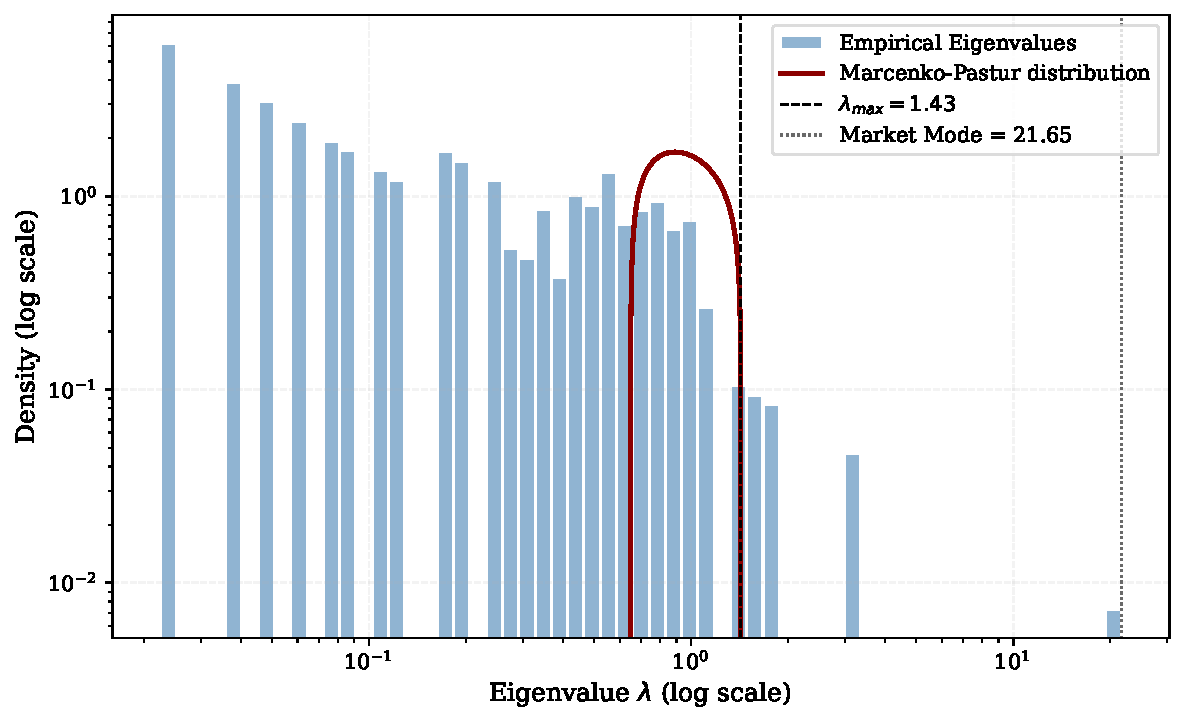
\includegraphics[width=0.85\linewidth]{images/figure_6_rmt_eigenvalue_spectrum.pdf}
\captionof{figure}{Empirical eigenvalue spectrum and Mar\v{c}enko--Pastur bounds. The largest eigenvalue is far outside the random band and captures the market-mode component.}
\label{fig:rmt_spectrum}
\end{center}

Figure~\ref{fig:rmt_filtered_matrices} shows the effect of this separation. The original matrix is dominated by broadly positive correlations, consistent with the strong collective component identified in the eigenspectrum. After removal of the leading mode, the candidate group-mode component reveals a more heterogeneous pattern, with localized positive and negative contrasts that were less visible in the original matrix.
\begin{center}
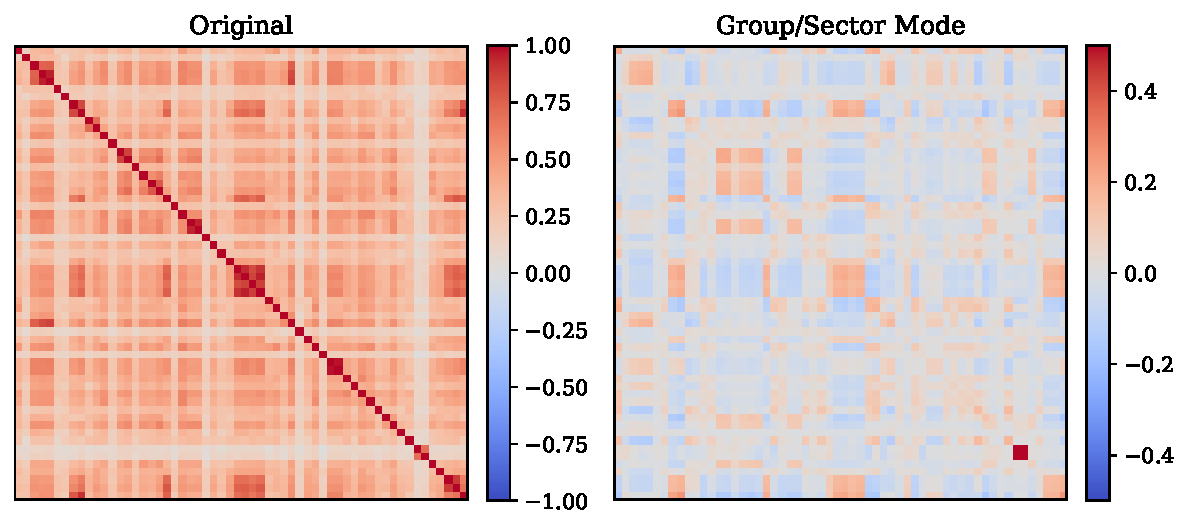
\includegraphics[width=0.9\linewidth]{images/figure_8_original_group_matrices.pdf}
\captionof{figure}{Original and candidate group-mode RMT component matrices at readable scale. The original matrix is dominated by broad positive co-movement, whereas the group-mode component highlights weaker localized contrasts after the leading market mode is removed.}
\label{fig:rmt_filtered_matrices}
\end{center}

The persistence of structured contrasts after market-mode removal suggests that the significant non-leading modes are not merely weaker copies of the collective component. Their composition must therefore be examined directly through their eigenvector loadings before determining whether the same organization reappears in hierarchical and network representations.

\subsubsection{Composition of the Significant Spectral Modes}

Eigenvalues indicate the strength of collective modes, while their eigenvectors reveal how individual assets contribute to each component. Figure~\ref{fig:eigenvector_loadings} reports the largest loadings for the five eigenvalues above the Mar\v{c}enko--Pastur upper bound. Assets are ranked by loading magnitude within each eigenvector. Because the overall sign of an eigenvector is arbitrary, the interpretation focuses on the relative contrasts, magnitude, and concentration of the loadings.

\begin{center}
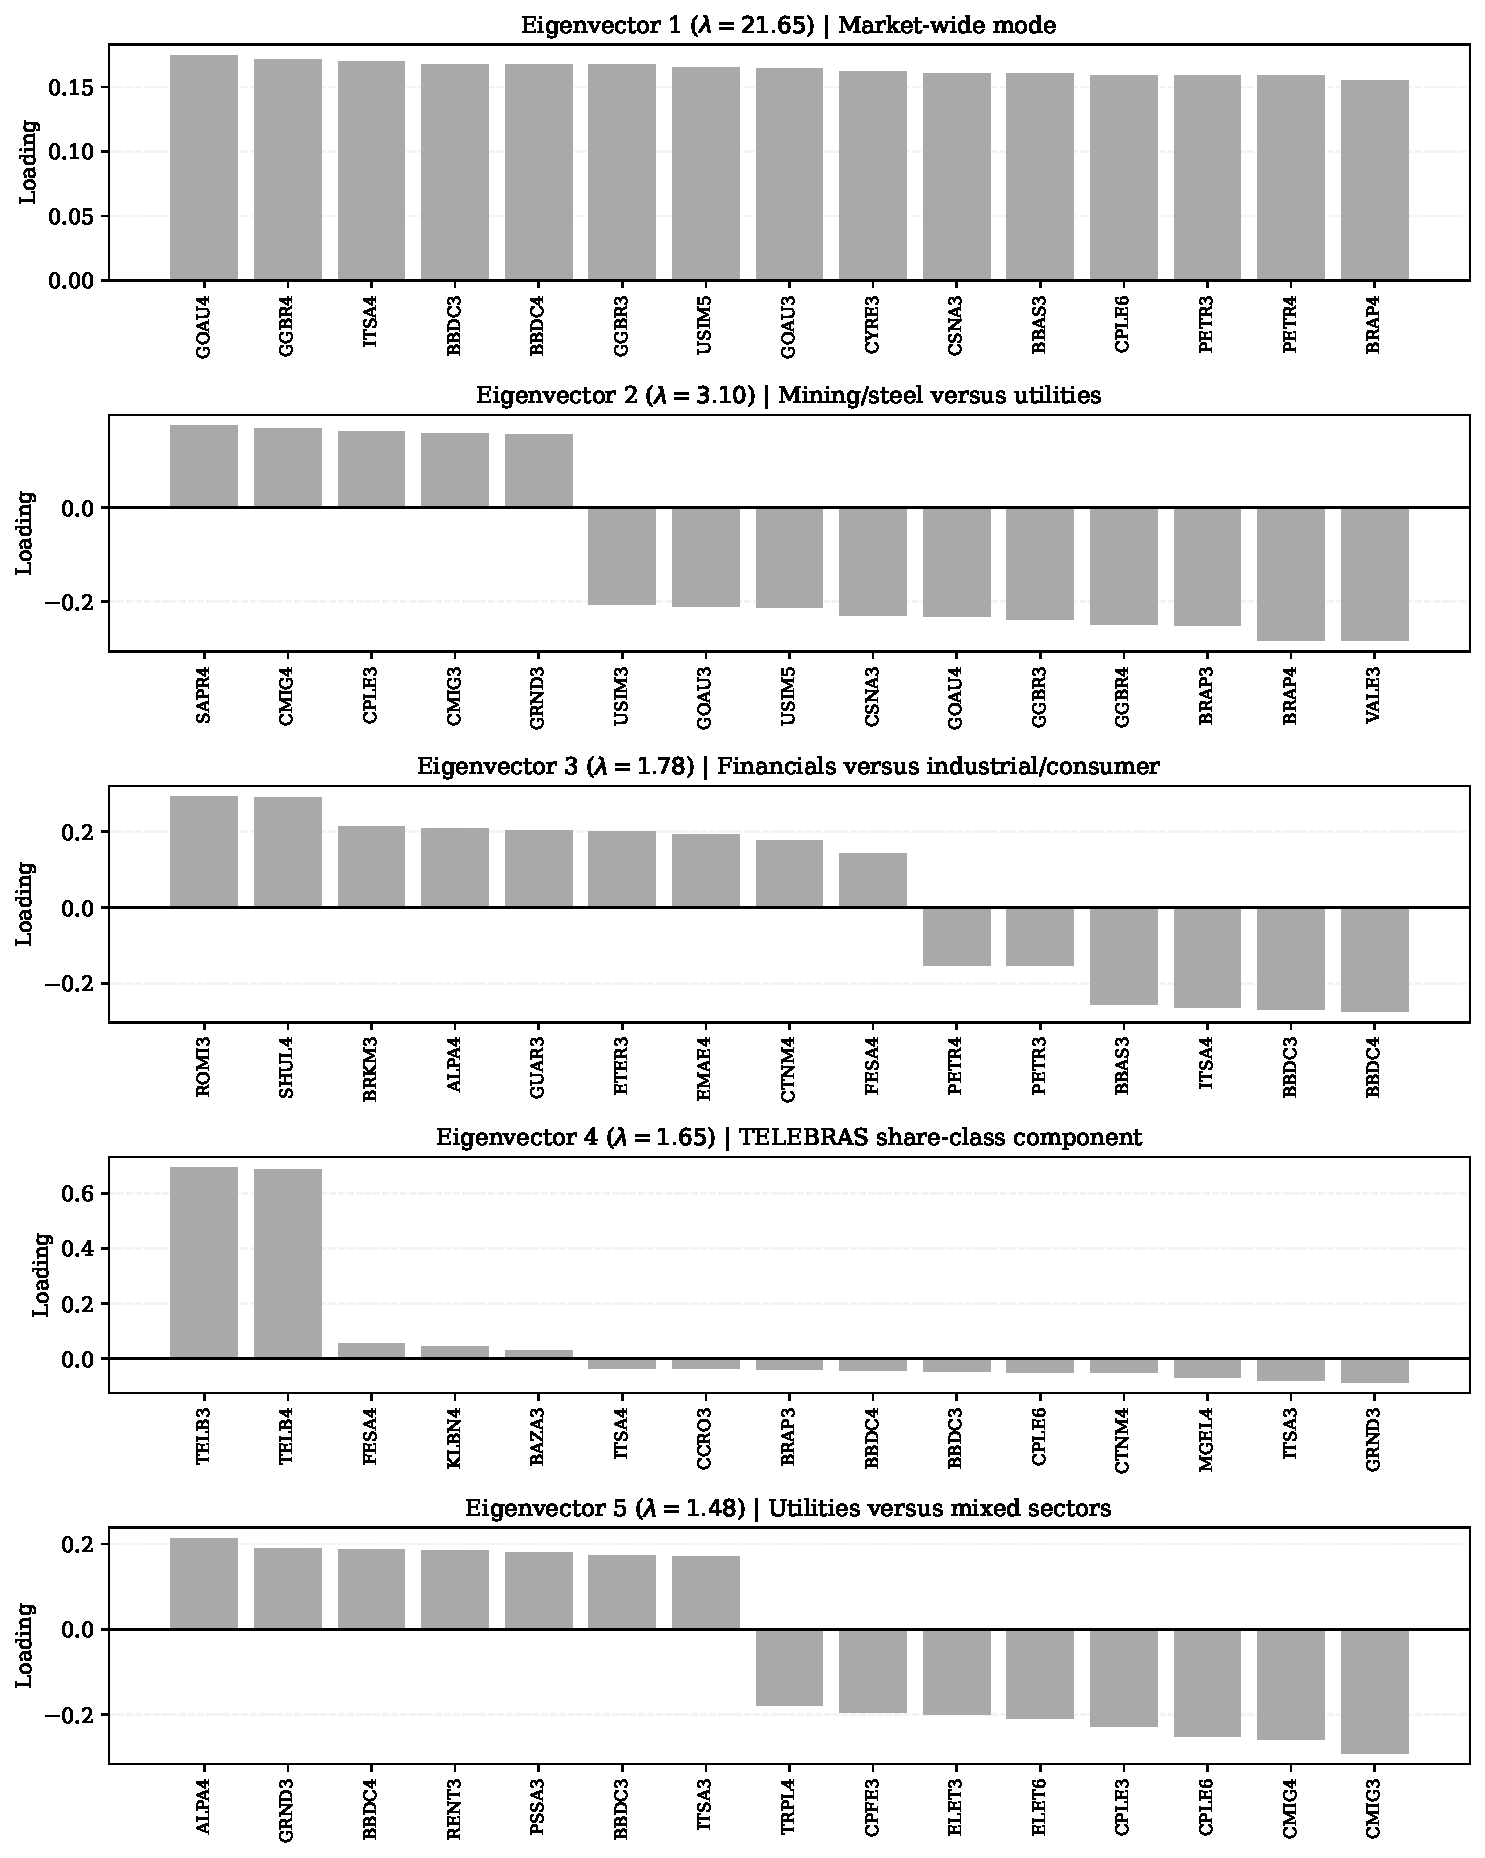
\includegraphics[width=0.95\linewidth]{images/figure_7b_rmt_top_eigenvectors_top_loadings.pdf}
\captionof{figure}{Top eigenvector loadings for the five RMT modes above the Mar\v{c}enko--Pastur upper bound. Eigenvector 1 is a broad market mode. Subsequent eigenvectors show relative contrasts between groups of assets; their overall signs are arbitrary.}
\label{fig:eigenvector_loadings}
\end{center}

The first eigenvector exhibits positive loadings across all 58 assets, ranging from 0.037 to 0.174. Its contribution is distributed across multiple sectors rather than concentrated in a single economic group, reinforcing the interpretation of the leading component as a broad market mode.

The second eigenvector ($\lambda_2=3.10$) is best read as a relative contrast between mining and steel firms---including VALE3, BRAP3/4, GGBR3/4, GOAU3/4, CSNA3 and USIM3/5---and a group led by utilities and selected consumer-cyclical assets. It therefore contains a commodity-related dimension, but it is not a pure Basic Materials factor.

The third eigenvector ($\lambda_3=1.78$) similarly contrasts the financial pole formed by BBDC3/4, ITSA4 and BBAS3 with a more heterogeneous industrial, chemical and consumer-cyclical pole led by ROMI3, SHUL4, BRKM3, ALPA4 and GUAR3.

The fourth eigenvector ($\lambda_4=1.65$) is highly concentrated in TELB3 and TELB4, the two listed TELEBRAS share classes. We interpret this result as an issuer-specific share-class component, rather than as evidence of a broad telecommunications factor. 

The fifth eigenvector ($\lambda_5=1.48$) separates a coherent utilities block---including CEMIG, COPEL, Eletrobras, CPFL Energia and ISA CTEEP---from financial and selected consumer-cyclical assets. This is a plausible utilities-related pattern, but $\lambda_5$ lies only about 3.7\% above the Mar\v{c}enko--Pastur upper bound. Its economic interpretation should therefore remain cautious and be treated as a candidate localized mode.

Overall, Figure~\ref{fig:eigenvector_loadings} shows that the modes beyond the dominant market component are structured contrasts rather than simple one-sector classifications. Some modes align partially with recognizable economic groups, while others reflect more localized or issuer-specific relationships. This motivates the subsequent hierarchical and network analyses, which examine whether these spectral patterns reappear in alternative representations of the dependency structure.
